\clearpage
\section*{GUI}
\phantomsection\label{sec:gui}

L'interfaccia grafica permette di apprendere e visualizzare l'intero albero.
Non occorre rispondere alle domande della console: le condizioni e i valori
predetti sono mostrati direttamente nel grafico.

\subsection*{Avvio e primo training locale}

Aprire un terminale nella \textbf{cartella principale del progetto} ed eseguire:

\begin{lstlisting}
java -jar distribution/gui/mapGUI.jar
\end{lstlisting}

Si apre la finestra \textbf{Progetto Map 2026}. All'inizio è selezionata
l'origine \textbf{File locale}, la barra di stato indica \textbf{Pronto} e
l'area centrale mostra \textbf{In attesa del training}.

\begin{enumerate}
  \item Lasciare selezionato \textbf{File locale}.
  \item Nel campo \textbf{Training set} mantenere il percorso predefinito
        \path{distribution/src/prova.dat}. In alternativa premere
        \textbf{Scegli file} e selezionare un training set \texttt{.dat}.
  \item Premere \textbf{Avvia training} e attendere il risultato. Non è
        necessario avviare il server o installare MySQL per questa modalità.
\end{enumerate}

\begin{center}
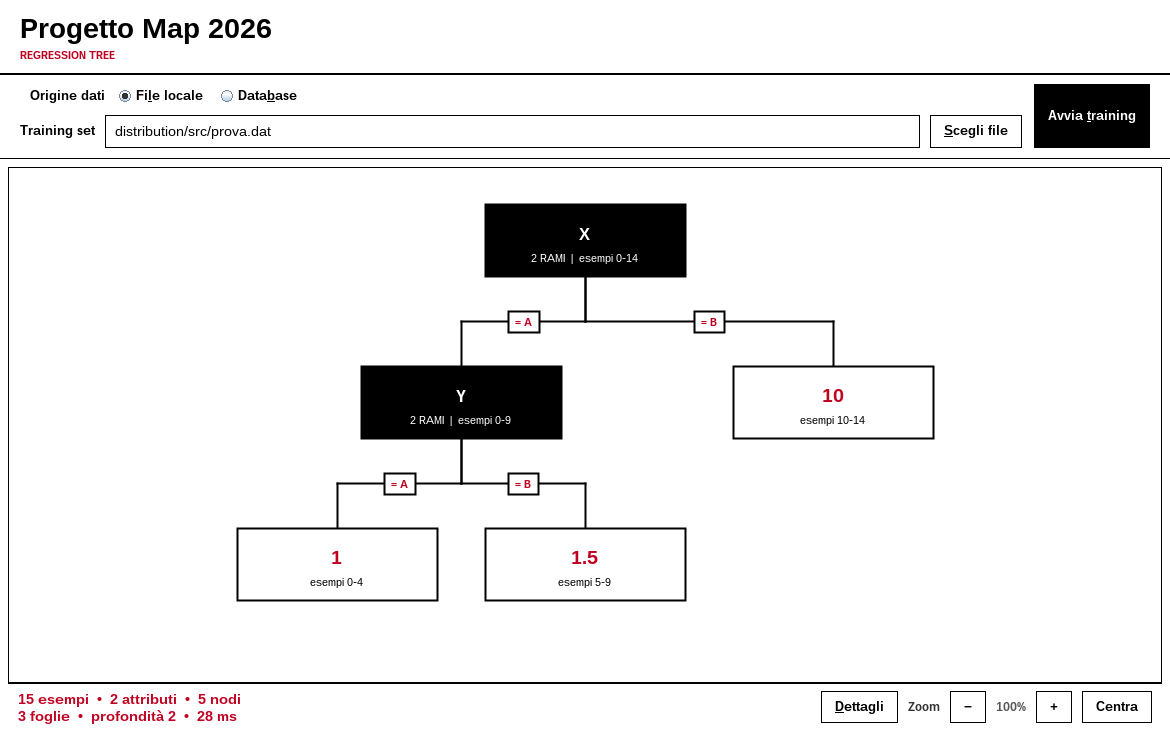
\includegraphics[width=\textwidth]{immagini/gui-locale.png}
\end{center}
\didascalia{GUI dopo il training locale su prova.dat. L'aspetto dei controlli
può variare con il sistema operativo; il tempo visualizzato dipende dalla macchina.}

Per questo file il risultato comprende \textbf{15 esempi}, \textbf{2 attributi},
\textbf{5 nodi}, \textbf{3 foglie} e \textbf{profondità 2}. Il pulsante
\textbf{Dettagli} diventa disponibile. Se il percorso predefinito non viene
trovato, avviare il programma dalla cartella principale oppure scegliere il
file tramite il selettore, che inserisce il percorso assoluto.

\clearpage
\subsection*{Lettura dell'albero e dei risultati}

L'albero si legge dall'alto verso il basso. I rettangoli \textbf{neri}
rappresentano gli attributi su cui si effettuano le scelte. I rettangoli
\textbf{bianchi}, con il valore numerico in rosso, sono le foglie e contengono
la predizione. Le etichette sui collegamenti indicano la condizione da seguire.

Per il file locale \texttt{prova.dat}, gli attributi \texttt{X} e \texttt{Y}
sono discreti. Le predizioni si leggono così:

\begin{center}
\begin{tabularx}{\textwidth}{@{}Xr@{}}
\toprule
\textbf{Percorso} & \textbf{Valore predetto} \\
\midrule
\texttt{X=A}, poi \texttt{Y=A} & 1 \\
\texttt{X=A}, poi \texttt{Y=B} & 1.5 \\
\texttt{X=B} & 10 \\
\bottomrule
\end{tabularx}
\end{center}

Il grafico è una \textbf{visualizzazione}, non un modulo di inserimento per
nuovi esempi: i nodi non sono pulsanti e non si selezionano con un clic.
Per una predizione guidata tramite domande usare il client da console.
I valori delle foglie sono mostrati con al massimo quattro cifre decimali.

\subsection*{Comandi di consultazione}

\begin{center}
\begin{tabularx}{\textwidth}{@{}lX@{}}
\toprule
\textbf{Comando} & \textbf{Effetto} \\
\midrule
\textbf{Dettagli} & Apre la finestra \textbf{Dettagli albero} con la
rappresentazione testuale del risultato. È disponibile dopo un training riuscito. \\
\textbf{Zoom -- / +} & Riduce o aumenta lo zoom di 10 punti percentuali,
fra 50\% e 150\%. La percentuale corrente è indicata accanto ai pulsanti. \\
\textbf{Centra} & Riporta la vista verso la radice, in alto. Non adatta
l'intero albero alla finestra e non reimposta lo zoom. \\
\textbf{Barre di scorrimento} & Permettono di esplorare gli alberi che
superano l'area visibile. Compaiono quando necessarie. \\
\bottomrule
\end{tabularx}
\end{center}

La barra inferiore riporta nodi, foglie, profondità e tempo impiegato.
La profondità è il numero massimo di collegamenti dalla radice a una foglia:
un albero formato da una sola foglia ha profondità zero. Il tempo indicato
non è una stima del tempo restante.

In modalità locale sono mostrati anche numero di esempi e attributi. La
scritta \texttt{esempi 0-14}, per esempio, indica un intervallo di indici nei
dati elaborati: durante il training gli esempi vengono riordinati, quindi non
si tratta dei numeri di riga originali del file.

Per apprendere un altro albero, cambiare file oppure origine e premere
nuovamente \textbf{Avvia training}. Il nuovo risultato sostituisce quello
precedente; il semplice cambio dell'origine non avvia alcuna elaborazione.

\clearpage
\subsection*{Training da database}

Questa modalità richiede MySQL configurato e il \textbf{server MAP già
avviato}, come descritto all'inizio del manuale. La GUI comunica con il server
MAP: non si collega direttamente alla porta MySQL e non richiede credenziali
del database nella finestra.

\begin{enumerate}
  \item Selezionare \textbf{Database} in \textbf{Origine dati}.
  \item Nel campo \textbf{Tabella} inserire \texttt{provaC}, oppure il nome
        di un'altra tabella compatibile già presente in \texttt{MapDB}.
        Non inserire un percorso, un comando SQL o il suffisso \texttt{.dat}.
  \item Nel campo \textbf{Server MAP} inserire \texttt{localhost} se il
        server è sullo stesso computer; altrimenti usare il suo indirizzo.
  \item Nel campo accanto ai due punti inserire la porta del server MAP,
        normalmente \texttt{8080}, \textbf{non 3306}, che è la porta MySQL.
  \item Premere \textbf{Avvia training} e attendere la comparsa dell'albero.
\end{enumerate}

\begin{center}
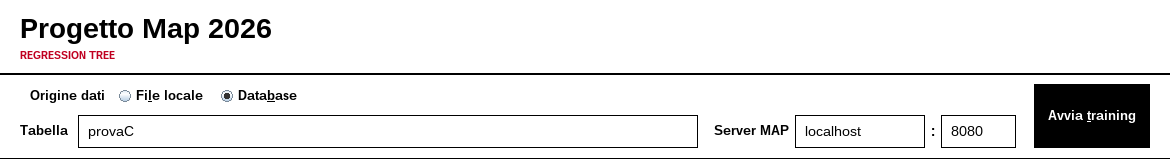
\includegraphics[width=\textwidth]{immagini/gui-database.png}
\end{center}
\didascalia{Pannello di configurazione dell'origine Database con i valori predefiniti.}

La tabella deve avere un nome che inizia con una lettera; i caratteri
successivi possono essere lettere, cifre, underscore o dollaro. La porta deve
essere un intero fra 1 e 65535. La configurazione JDBC del server usa
\texttt{localhost:3306/MapDB}, utente \texttt{MapUser} e password \texttt{map},
coerentemente con lo script di prima installazione fornito.

Al termine, la barra riporta tabella, server, numero di nodi e foglie,
profondità e tempo. Non mostra il numero degli esempi e degli attributi,
perché queste informazioni non vengono trasferite dal protocollo remoto.
\textbf{Dettagli} visualizza il nome della tabella e la struttura ricostruita.

\subsection*{Esempio con la tabella provaC}

Nella tabella \texttt{provaC} fornita dallo script, \texttt{X} è discreto e
\texttt{Y} è numerico. Diversamente da \texttt{prova.dat}, il secondo split
utilizza una soglia:

\begin{center}
\begin{tabularx}{\textwidth}{@{}Xr@{}}
\toprule
\textbf{Percorso} & \textbf{Valore predetto} \\
\midrule
\texttt{X=A}, poi \texttt{Y<=2.0} & 1 \\
\texttt{X=A}, poi \texttt{Y>2.0} & 1.5 \\
\texttt{X=B} & 10 \\
\bottomrule
\end{tabularx}
\end{center}

Il server salva automaticamente \texttt{provaC.dmp} nella propria directory
di lavoro, sovrascrivendo l'eventuale archivio omonimo. La GUI non salva una
copia sul computer del client e non permette di aprire direttamente gli
archivi: per riutilizzarli senza apprendere di nuovo, usare l'opzione
\textbf{2} della CLI.

\clearpage
\subsection*{Formato dei training set locali}

\textbf{Scegli file} seleziona un dataset di testo \texttt{.dat}, non un albero
serializzato \texttt{.dmp} e non un file CSV generico privo di schema.
Il seguente esempio riproduce il contenuto di \texttt{prova.dat} distribuito:

\begin{lstlisting}
@schema 2
@desc X A,B,C,D,E
@desc Y A,B,C,D,E
@target class
@data 15
A,A,1
A,A,1
A,A,1
A,A,1
A,B,1.5
A,B,1.5
A,B,1.5
B,B,10
A,B,1.5
A,B,1.5
B,C,10
B,B,10
B,C,10
B,C,10
A,A,1
\end{lstlisting}

\begin{itemize}
  \item \texttt{@schema 2} indica due attributi descrittivi, escluso il target.
  \item Ogni \texttt{@desc} dichiara un attributo. L'elenco separato da
        virgole specifica il dominio discreto; senza elenco l'attributo è
        continuo. Per esempio, \texttt{@desc Y} dichiara \texttt{Y} numerico.
  \item \texttt{@target class} dichiara il nome del target numerico,
        collocato nell'ultima colonna di ogni riga.
  \item \texttt{@data 15} dichiara esattamente quindici esempi. Ogni riga
        contiene i valori degli attributi nell'ordine dello schema, poi
        il target; i campi sono separati da virgole.
\end{itemize}

Usare il \textbf{punto} come separatore decimale, rispettare maiuscole e
minuscole dei valori discreti e non aggiungere righe vuote o commenti.
Nelle dichiarazioni usare un singolo spazio fra i campi, come nell'esempio.
Il numero di righe e quello delle colonne devono coincidere con lo schema.

Sono disponibili anche \path{distribution/src/provaC.dat}, con un
attributo continuo, e \path{distribution/src/servo.dat}, più ampio.
I file non vengono modificati dal training. La modalità locale conserva il
risultato soltanto in memoria e non crea un archivio \texttt{.dmp}.

\subsection*{Chiusura}

Chiudere la finestra per terminare la GUI. Il risultato locale non viene
salvato automaticamente; se serve nuovamente, ripetere il training sul file.
Il server MAP resta attivo anche dopo la chiusura della GUI o della CLI:
per arrestarlo, premere \textbf{Ctrl+C} nel suo terminale.
